%%%%%%%%%%%%%%%%%%%%%%%%%%%%%%%%%%%%%%%%%
%
% (c) 2022 by Jennifer Laaser
%
% This work is licensed under the Creative Commons Attribution-NonCommercial-ShareAlike 4.0 International License. To view a copy of this license, visit http://creativecommons.org/licenses/by-nc-sa/4.0/ or send a letter to Creative Commons, PO Box 1866, Mountain View, CA 94042, USA.
%
% The current source for these materials is accessible on Github: https://github.com/jlaaser/pogil-polymers
%
%%%%%%%%%%%%%%%%%%%%%%%%%%%%%%%%%%%%%%%%%

\renewcommand{\figpath}{content/polymphys/solution-thermo/flory-huggins/figs}
\renewcommand{\labelbase}{flory-huggins}

\begin{activity}{Regular Solutions \& Flory-Huggins Theory}

\begin{instructornotes}

	This activity introduces students to key concepts related to polymer solutions, including ideal mixing, regular solution theory, and Flory-Huggins theory.
	
	After completing this activity, students will be able to:
			\begin{enumerate}
				\item Explain why mixing is said to be an entropy-driven process (ideal solutions)
				\item Explain how enthalpic interactions change the free energy of mixing (regular solutions)
				\item Explain the origin of the $1/N$ term in the Flory-Huggins free energy of mixing for polymer solutions
			\end{enumerate}
	This activity will prepare students for follow-up activities on phase diagrams for polymer solutions.
			
	\subsection*{Activity summary:}
	\begin{itemize}
		\item \textbf{Activity type:} Learning Cycle
		\item \textbf{Content goals:} See above %Ideal mixing, regular solution theory, and Flory-Huggins theory
		\item \textbf{Process goals:} %https://pogil.org/uploads/attachments/cj54b5yts006cklx4hh758htf-process-skills-official-pogil-list-2015-original.pdf
			\begin{itemize}
				\item Interpreting equations and figures
				\item Applying equations to describe a model
				\item Written and oral communication of reasoning
			\end{itemize}
		\item \textbf{Duration:} approx. 75 minutes, including class discussion
		
			\emph{Note: this activity is long, and can be split across two days if necessary.  The best split point is at the end of Model 1; in this case, Model 1 takes approximately 30 minutes on the first day, and Models 2 \& 3 take approximately 30-40 minutes on the second day. Students can also be asked to complete CTQs 1 and 2 before class as a warm-up exercise, and the remainder of the activity can then be completed in class in approx. 50 minutes.}
			
			\emph{If needed, the content at the beginning of Model 2 (CTQs 9-11) also lends itself well to being presented in a mini lecture, with students picking up at CTQ 12.}
			
		\item \textbf{Instructor preparation required:} none beyond knowledge of relevant content
		\item \textbf{Related textbook chapters:}
			\begin{itemize}
				\item \emph{Polymer Chemistry} (Hiemenz \& Lodge), 2nd ed.: sections 7.1-7.3
				\item \emph{Introduction to Polymers} (Young \& Lovell), 3rd ed.: sections 10.2.1 and 10.2.2
		\end{itemize}
	\end{itemize}

\end{instructornotes}

	%\textbf{Focus question:} Put a central question for the students to consider through this exercise here.

\begin{model}[Ideal Mixtures: A Toy Model]
\label{\labelbase:mdl:ideal}

A simple model for mixing of two small-molecule liquids is shown below.  In this model, each molecule is shown as a circle, and we place them in a grid where each molecule takes up exactly one ``space'' in the grid.

Initially, the molecules of each type are isolated in their own containers:

\centerline{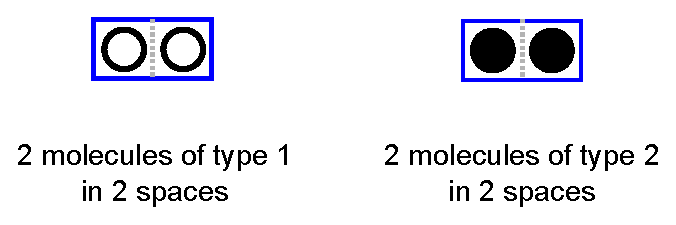
\includegraphics[width=0.6\textwidth]{\figpath/model1-initial}}

After combining the two containers, the molecules mix together:

\vspace{6pt}
\centerline{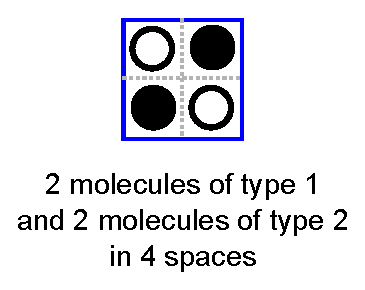
\includegraphics[width=0.3\textwidth]{\figpath/model1-mixed}}

The critical elements of this model are that
\begin{enumerate}[itemsep=0pt,topsep=-6pt]
	\item the number of molecules of each type does not change,
	\item the molecules each take up exactly the same volume (here, one square on the grid),
	\item the total volume after mixing is the sum of the two initial volumes, and
	\item the mixing is entirely random.
\end{enumerate}

\end{model}

\vspace{0.05in}
\begin{ctqs}

	\question Consider the simple system shown in Model \ref{\labelbase:mdl:ideal}, which contains two molecules of type 1 and two molecules of type 2: \label{\labelbase:ctq:toyconfigs}
	
		\begin{enumerate}
			\item How many different ways can you distribute the two molecules of type 1 in their initial box, assuming the molecules are indistinguishable (you can't tell them apart)?  Sketch the possible configurations below.  Note that you may not need to use all of the boxes; cross off any you don't need.
			
				\begin{solution}
					\studentdisplay{

\centerline{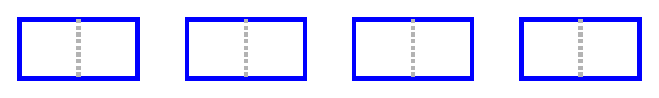
\includegraphics[width=0.6\textwidth]{\figpath/model1-2blank}}

						\vspace{0.1in}
						\centerline{Number of configurations ($\Omega_1$) = $\rule{1cm}{0.15mm}$}
					}
					\instructordisplay{

\centerline{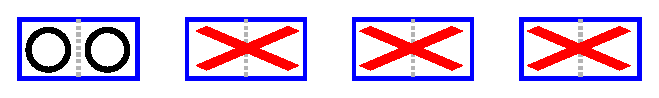
\includegraphics[width=0.6\textwidth]{\figpath/model1-2solution-type1}}

						\vspace{0.1in}
						\centerline{Number of configurations ($\Omega_1$) = 1}
					}
				\end{solution}
		
			\item How many different ways can you distribute the two molecules of type 2 in their initial box, assuming the molecules are indistinguishable (you can't tell them apart)?  Sketch the possible configurations below. Again, you may not need to use all of the boxes.
			
				\begin{solution}
					\studentdisplay{

\centerline{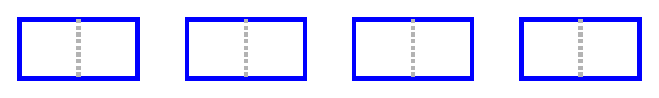
\includegraphics[width=0.6\textwidth]{\figpath/model1-2blank}}

						\vspace{0.1in}
						\centerline{Number of configurations ($\Omega_2$) = $\rule{1cm}{0.15mm}$}
					}
					\instructordisplay{

\centerline{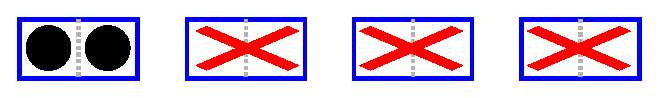
\includegraphics[width=0.6\textwidth]{\figpath/model1-2solution-type2}}

						\vspace{0.1in}
						\centerline{Number of configurations ($\Omega_2$) = 1}
					}
				\end{solution}
			
			\item How many different ways can you distribute the four molecules in the final mixture, assuming that you can't distinguish molecules of the same type from each other?  Sketch them below.  Again, you may not need to use all of the boxes.
			
				\begin{solution}
					\studentdisplay{

\centerline{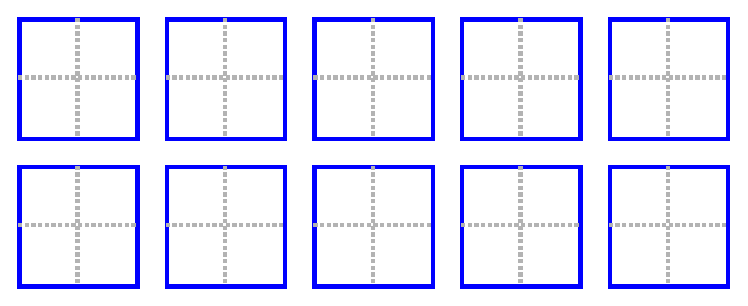
\includegraphics[width=0.6\textwidth]{\figpath/model1-4blank}}

						\vspace{0.1in}
						\centerline{Number of configurations ($\Omega_{mixed}$) = $\rule{1cm}{0.15mm}$}
					}
					\instructordisplay{

\centerline{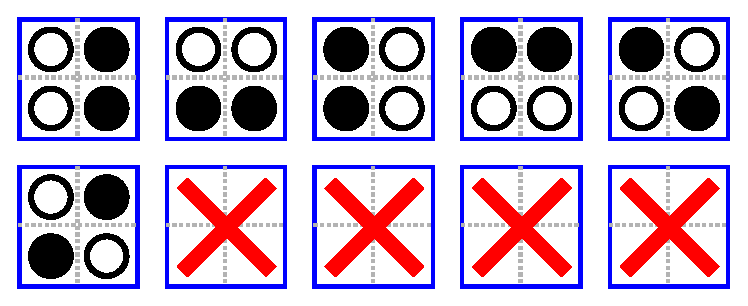
\includegraphics[width=0.6\textwidth]{\figpath/model1-4solution}}

						\vspace{0.1in}
						\centerline{Number of configurations ($\Omega_{mixed}$) = 6}
					}
				\end{solution}
		\end{enumerate}
		
	\question Recall that if $\Omega$ is the number of ways that the molecules in the system can be arranged, then the entropy of that system is given by
		\begin{equation*}
			S = k_B \ln \Omega
		\end{equation*} 
		where $k_B$ is the Boltzmann constant.  Using this relationship, and your answers from CTQ \ref{\labelbase:ctq:toyconfigs}, calculate
			
		\begin{enumerate}
			\item the entropy of the initial state ($S_{initial} = S_1 + S_2$, where $S_1 = k_B\ln \Omega_1$ and $S_2 = k_B \ln \Omega_2$):
			
				\begin{solution}[1in]
					\begin{align*}
						S_{initial} &= S_1 + S_2 \\
							&= k_B\ln\Omega_1 + k_B\ln\Omega_2\\
							&= k_B \ln 1 + k_B \ln 1 \\
							&= k_B\cdot 0 + k_B\cdot 0 = 0
					\end{align*}
				\end{solution}
				
			\item the entropy of the final (mixed) state, $S_{mixed}$:
			
				\begin{solution}[0.75in]
					\begin{align*}
						S_{mixed} &= k_B\ln\Omega_{mixed} \\
							&= k_B \ln 6
					\end{align*}
				\end{solution}
				
			\item the change in entropy upon mixing ($\Delta S_{mix} = S_{mixed} - S_{initial}$): 
			
				\begin{solution}[0.75in]
					\begin{align*}
						\Delta S_{mix} &= S_{mixed} - S_{initial} \\
							&= k_B \ln 6 - 0\\
							&= k_B \ln 6
					\end{align*}
				\end{solution}
				
		\end{enumerate}
		
\end{ctqs}

\begin{infobox}

	A more general case of the mixing process described in Model \ref{\labelbase:mdl:ideal} is shown below:
	
	\centerline{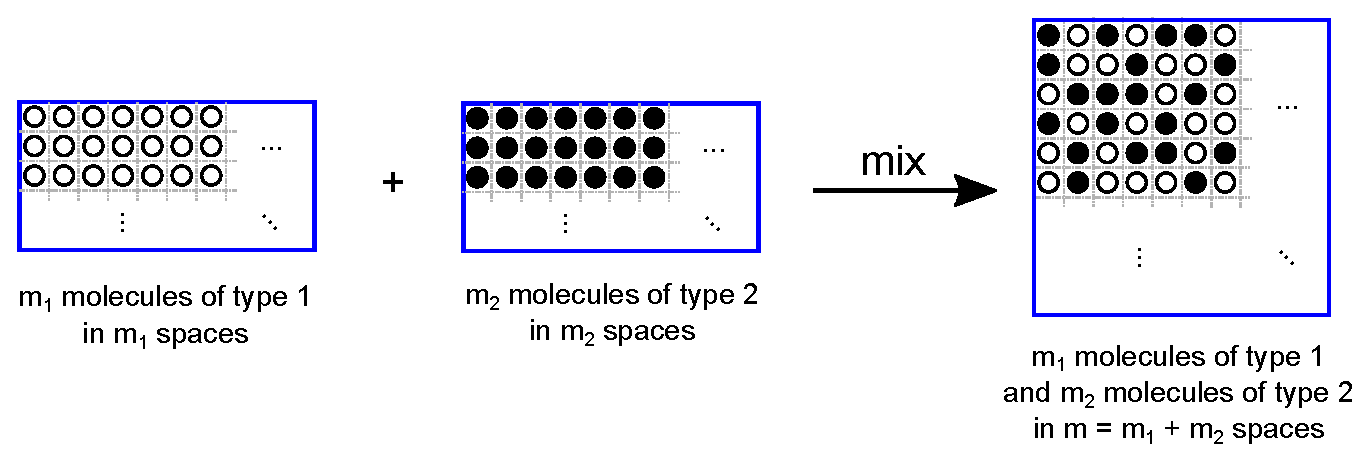
\includegraphics[width=0.8\textwidth]{\figpath/model2-mixing}}
	
	For this general case, it is possible to show (see Exercise \ref{\labelbase:exc:idealmixing}) that the entropy of mixing is 
	\begin{equation*}
		\Delta S_{mix} = -k_B\left(m_1 \ln\left(\frac{m_1}{m}\right) + m_2 \ln\left(\frac{m_2}{m}\right) \right) \label{\labelbase:eqn:idealS}
	\end{equation*}
\end{infobox}

\begin{ctqs}

	\question If you were to double both $m_1$ and $m_2$ (thus doubling the total number of molecules, $m$, while keeping the ratio of type-1 and type-2 molecules the same), what would happen to the value of $\Delta S_{mix}$?
	
		\begin{solution}[1in]
		
			$\Delta S_{mix}$ would double.  If we replace $m_1$, $m_2$, and $m$ with twice their original values, $\Delta S_{mix}$ becomes
			\vspace{-6pt}
			\begin{align*}
				\Delta S_{mix,doubled} &= -k_B\left(2m_1 \ln\left(\frac{2m_1}{2m}\right) + 2m_2 \ln\left(\frac{2m_2}{2m}\right) \right)\\
				 &= -k_B\left(2m_1 \ln\left(\frac{m_1}{m}\right) + 2m_2 \ln\left(\frac{m_2}{m}\right) \right)\\
				 %&= 2\left[-k_B\left(m_1 \ln\left(\frac{m_1}{m}\right) + m_2 \ln\left(\frac{m_2}{m}\right) \right)\right]\\
				 &= 2\Delta S_{mix}
			\end{align*}
		\end{solution}
	
	
	\question Recall that \emph{extensive} properties are properties that depend on the total number of molecules in the system, while \emph{intensive} properties do not depend on the total number of molecules present.
	
	Based on your answer to the previous question, is $\Delta S_{mix}$ an intensive or extensive property?
	
		\begin{solution}[0.5in]
		
			Extensive - the value of $\Delta S_{mix}$ changes when we change the total number of molecules present.
		
		\end{solution}
	
	\question Usually, it is most convenient to divide by the total number of molecules, which leaves us with an intensive expression for the entropy, 
		\begin{equation*}
			\Delta S_{mix}^{(int)} = \frac{1}{m} \Delta S_{mix}
		\end{equation*}
		Using this expression, and the equation for $\Delta S_{mix}$ given above, write an expression for $\Delta S_{mix}^{(int)}$ in terms of $m_1$, $m_2$, and $m$.
		
			\begin{solution}[0.75in]
			
				\begin{equation*}
					\Delta S_{mix}^{(int)} = -k_B\left(\frac{m_1}{m} \ln\left(\frac{m_1}{m}\right) + \frac{m_2}{m} \ln\left(\frac{m_2}{m}\right) \right)
				\end{equation*}
			\end{solution}
		
	\question We also often prefer to work in terms of \emph{mole fractions} rather than numbers of molecules. \label{ctq:Smixed}
	
		Rewrite your expression for $\Delta S_{mix}^{(int)}$ in terms of the mole fractions
		\begin{align*}
			x_1 = \frac{m_1}{m_1 + m_2} = \frac{m_1}{m} && \text{and} && x_2 = \frac{m_2}{m_1+m_2} = \frac{m_2}{m}
		\end{align*}
		
			\begin{solution}[0.75in]
			
				\begin{equation*}
					\Delta S_{mix}^{(int)} = -k_B\left(x_1 \ln x_1 + x_2 \ln x_2 \right)
				\end{equation*}
			\end{solution}
		
	\question The mole fractions, $x_1$ and $x_2$, must both be between 0 and 1.  In this case,
		\begin{enumerate}
			\item Will $\ln x_1$ (and $\ln x_2$) be positive or negative?
	
				\begin{solution}[1in]
					negative
				\end{solution}
				
			\item Will $\Delta S_{mix}^{(int)}$ be positive or negative? \label{ctq:Spositive}
	
				\begin{solution}[1in]
					positive (there is a negative sign out front, which cancels the negative value of the logarithms)
				\end{solution}
				
		\end{enumerate}
		
	\question Explain, in 1-2 complete sentences, why we say that ideal mixing is an \emph{entropy-driven} process.
	
		\begin{solution}[2.5in]
		
			As shown above, the entropy change upon mixing is positive.  Generally, processes that increase entropy are favorable, so the increase in entropy makes it favorable for mixing to occur.
			
			Students may also answer in terms of $\Delta G$: since $\Delta G = \Delta H - T\Delta S$, putting a positive value of $\Delta S$ in makes $\Delta G$ more negative, making the mixing process more favorable.
		\end{solution}
		
\end{ctqs}
	
\clearpage
\begin{model}[Real Mixtures: Enthalpy of Mixing]
\label{\labelbase:mdl:regular}

In \emph{ideal} mixtures, such as those described in Model \ref{\labelbase:mdl:ideal}, the molecules do not interact with each other, and entropy is the only thermodynamic consideration that affects mixing.
In \emph{real} mixtures, however, molecules do interact with each other, and we must take those interactions into account when determining whether mixing is favorable or unfavorable.

To incorporate the energetics of intermolecular interactions into our model, we must make two key assumptions:
\begin{enumerate}
	\item First, we assume that molecules interact only with their immediate neighbors, and that each interaction involves only two molecules.  The interaction energies between different types of pairs are as follows:

\centerline{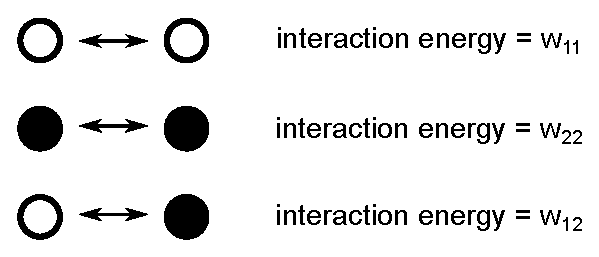
\includegraphics[width=0.4\textwidth]{\figpath/model3-interactions}}
	
	\item Second, we assume that each molecule has some specific number of neighbors, $z$, which we refer to as the ``coordination number''.  For example, the central molecule shown below has 4 nearest neighbors, so its coordination number is 4:

\centerline{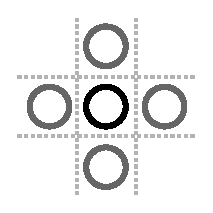
\includegraphics[width=0.15\textwidth]{\figpath/model3-coordnum}}

		Note that when drawing the molecules on a square lattice like this, we do not count molecules positioned diagonally from each other as being ``neighbors'' - molecules only interact with molecules that share a side of a square with them.

\end{enumerate}

\end{model}

\begin{ctqs}

	\question Before mixing, molecules are surrounded by molecules of only the same type, as shown below. \label{\labelbase:ctq:unmixedenthalpy}
	
		\centerline{\includegraphics[width=0.3\textwidth]{\figpath/Model3-unmixed}}	
	
		For this configuration, determine...
		\begin{enumerate}	
			\item ... the total number of 1-1 interactions:
				\begin{solution}[0.25in]
					4
				\end{solution}
			
			\item ... the total number of 2-2 interactions:
				\begin{solution}[0.25in]
					4
				\end{solution}
			
			\item ... the total number of 1-2 interactions:
				\begin{solution}[0.25in]
					0
				\end{solution}
			
			\item ... the total energy arising from interactions between the central molecules and their neighbors:
				\begin{solution}[0.25in]
					$4w_{11} + 4w_{22}$
				\end{solution}
			
		\end{enumerate}
		
	\question After mixing, molecules may be surrounded by molecules of a different type.  A simple ``mixed'' state, in which the central molecules have been swapped, is shown below: \label{\labelbase:ctq:mixedenthalpy}
	
		\centerline{\includegraphics[width=0.3\textwidth]{\figpath/Model3-mixed}}
	
		For this configuration, determine:
		\begin{enumerate}	
			\item ... the total number of 1-1 interactions:
				\begin{solution}[0.25in]
					0
				\end{solution}
			
			\item ... the total number of 2-2 interactions:
				\begin{solution}[0.25in]
					0
				\end{solution}
			
			\item ... the total number of 1-2 interactions:
				\begin{solution}[0.25in]
					8
				\end{solution}
			
			\item ... the total energy arising from interactions between the central molecules and their neighbors:
				\begin{solution}[0.25in]
					$8w_{12}$
				\end{solution}
			
		\end{enumerate}
	
	\question What is the \emph{change} in energy that occurs as the system goes from the un-mixed state in CTQ \ref{\labelbase:ctq:unmixedenthalpy} to the mixed state in CTQ \ref{\labelbase:ctq:mixedenthalpy}?
	
		\begin{solution}[0.75in]
			$8w_{12}-4w_{11}-4w_{22}$
		\end{solution}
	
	\question Explain, in 1-2 complete sentences, why $\Delta w = w_{12} - \frac{w_{11}}{2} - \frac{w_{22}}{2}$ (called the ``exchange energy'') can be interpreted as the energetic cost for breaking up interactions between like molecules to create new interactions between un-like molecules.
	
		\begin{solution}[1.75in]
			The molecules start only surrounded by neighbors of the same type.  Every time we create a new ``1-2'' interaction, it requires us to remove (break apart) some of the interactions between like molecules, which requires an energy input of $w_{11}$ or $w_{22}$ per interaction that we break apart. We then gain energy $w_{12}$ as we create the new interactions.  The factor of 1/2 is necessary because we essentially have to break half of a 1-1 interaction and half of a 1-2 interaction to create a single new 1-2 interaction.
		\end{solution}
		
\end{ctqs}

\begin{infobox} \label{\labelbase:eqn:Hmix}
It is possible to show (see Exercise \ref{\labelbase:exc:mixingenthalpy}) that, in general, the enthalpy of mixing for a sample containing both type-1 and type-2 molecules is given by
		\begin{align*}
			\Delta H_{mix}^{(int)} %&= \frac{m_1}{m}\frac{m_2}{m} z \left( w_{12} - \frac{w_{11}}{2} - \frac{w_{22}}{2}\right)  
					= x_1 x_2 z \Delta w %\label{\labelbase:eqn:Hmix}
		\end{align*}
		where $x_1$ and $x_2$ are the mole fractions of type-1 and type-2 molecules, respectively, and $\Delta w$ is the exchange energy defined above.
\end{infobox}

\begin{ctqs}

	\question It is common to normalize the total energy of the interaction  between a particle and its neighbors ($z\Delta w$) by the thermal energy, $k_BT$.  This normalized quantity is defined as the \emph{interaction parameter}, $\chi$:
		\begin{equation*}
			\chi = \frac{z\Delta w}{k_B T}
		\end{equation*}
	
		\begin{enumerate}
			\item Find an expression for $\Delta H_{mix}^{(int)}$ in terms of $x_1$, $x_2$, $\chi$, $k_B$, and $T$.
		
			\begin{solution}[0.5in]
				\begin{equation*}
					\Delta H_{mix}^{(int)} = x_1 x_2 \chi k_B T
				\end{equation*}
			\end{solution}

			\item Recalling that $\Delta G = \Delta H - T\Delta S$, combine this expression with your answer from question \ref{ctq:Smixed} to find an expression for $\Delta G_{mix}^{(int)}$.
			
			\begin{solution}[0.5in]
				\begin{align*}
					\Delta G_{mix}^{(int)} &= x_1 x_2 \chi k_B T + k_B T(x_1 \ln x_1 + x_2 \ln x_2)
				\end{align*}
			\end{solution}
		\end{enumerate}
			
		\question In question \ref{ctq:Spositive}, we noted that $\Delta S_{mix}^{(int)}$ is always positive, so the entropic term \emph{always} favors mixing.
		
			Given that $\chi$ is \emph{usually} (although not always) positive, does the enthalpic term usually favor mixing, or oppose it?  Briefly explain your answer in 1-2 complete sentences.
			
			\begin{solution}[2.5in]
			
				If $\chi$ is positive, then $\Delta H_{mix}$ will also be positive.  This increases the value of $\Delta G_{mix}$, which makes the process \emph{less} favorable.    Thus, when $\chi$ is positive (as it usually - but not always! - is), the enthalpic term opposes mixing.
				
			\end{solution}
\end{ctqs}

\begin{model}[Polymer Solutions]
\label{\labelbase:mdl:floryhuggins}

In Models \ref{\labelbase:mdl:ideal} and \ref{\labelbase:mdl:regular}, we considered mixtures of small molecules in which each molecule  was independent of the other molecules of the same type.

In polymers, however, this is no longer true: the monomers are linked together into polymer chains and must stay close to each other, as illustrated below: 
	
	\centerline{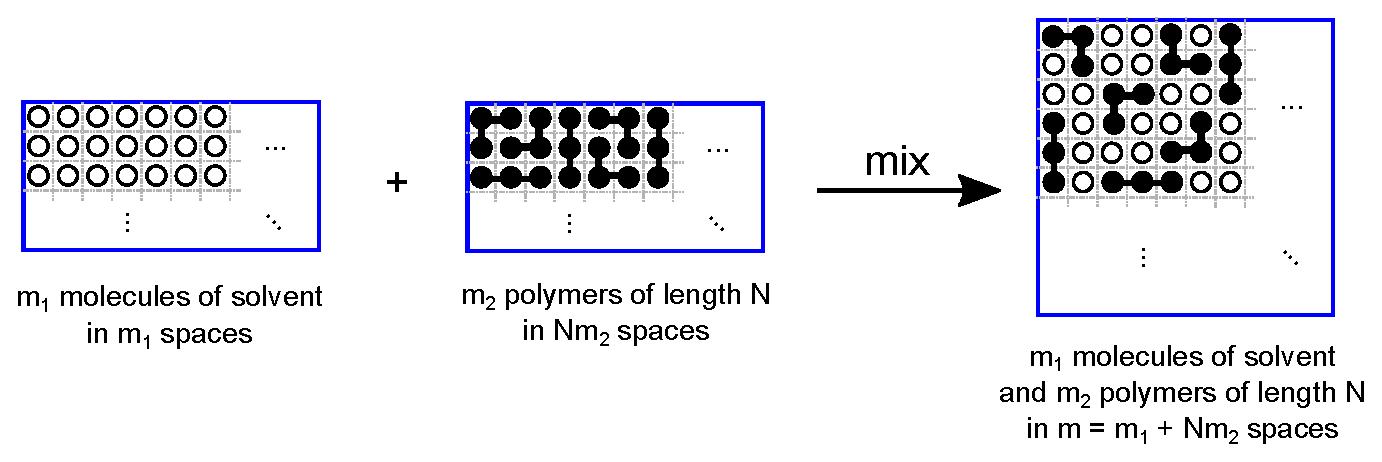
\includegraphics[width=\textwidth]{\figpath/model4-polymermixing}}

\end{model}

\begin{ctqs}

	\question \emph{On average}, when the type-2 molecules are linked into chains...
	
		\begin{enumerate}
			\item ... does it \emph{significantly} change the number of ways that the type-1 solvent molecules can be distributed in the final mixture?  Why or why not?
				\label{\labelbase:ctq:FHtype1}
			
				\begin{solution}[1in]
					No, linking the type-2 molecules into chains does not \emph{significantly} affect the number of ways that the type-1 (solvent) molecules can be distributed in the mixed state.  (The number of ways to distribute the type-1 molecules may change a little, but it is a small effect compared to the effect on the type-2 molecules addressed in the next question).
				\end{solution}
			
			\item ... does \emph{significantly} change the number of ways that the type-2 monomers can be distributed in the final mixture?  Why or why not?
				\label{\labelbase:ctq:FHtype2}
			
				\begin{solution}[0.9in]
					Yes, linking the type-2 monomers into chains does  significantly affect the number of ways that the monomer molecules can be distributed in the mixed state - because they are linked together, they are restricted to staying near each other in the final solution.
				\end{solution}
			
			\item ... does it \emph{significantly} change the total number of interactions between type-1 and type-2 molecules?  Why or why not?
				\label{\labelbase:ctq:FHinteraction}
			
				\begin{solution}[0.9in]
					No, linking the type-2 molecules into chains does not \emph{significantly} affect the number of interactions between type-1 and type-2 molecules in the mixed state.
				\end{solution}
				
		\end{enumerate}
	
\end{ctqs}

\begin{infobox}
	Flory-Huggins theory states that for a solution of $m_1$ solvent molecules (each of which takes up 1 space) and $m_2$ polymer molecules (each of which take up $N$ spaces) the free-energy of mixing is given by
	\begin{equation*}
		\frac{\Delta G_{mix}^{(int)}}{k_B T} = \underbrace{\phi_1 \phi_2 \chi}_{\text{enthalpic}} + \underbrace{\phi_1 \ln \phi_1 + \frac{\phi_2}{N} \ln \phi_2}_{\text{entropic}}
	\end{equation*}
	Note that this expression is given in terms of the \emph{volume fractions} ($\phi_1$ and $\phi_2$) of each component.  As in Models \ref{\labelbase:mdl:ideal} and \ref{\labelbase:mdl:regular}, $\phi_1$ and $\phi_2$ represent the \emph{fraction of boxes} filled by each type of molecule; however, since each polymer chain (which we count as a single molecule) fills more than one box, the fraction of boxes is no longer the same as the the mole fraction, so we use a different variable to denote it.
	
\end{infobox}

\begin{ctqs}

		\question Based on your answers to questions \ref{\labelbase:ctq:FHtype1}-\ref{\labelbase:ctq:FHinteraction}, why is the entropic contribution from the polymer molecules reduced by a factor of $1/N$ relative to the small molecule case? Explain your answer in 1-2 complete sentences.
		
			\begin{solution}[1.75in]
			
				The entropic contribution from the polymer molecules is reduced by a factor of $1/N$ because linking the monomers together reduces the number of ways that they can be distributed in the final mixture, thus reducing their increase in entropy upon mixing.
			
			\end{solution}
		
		\question Qualitatively, do you expect this $1/N$ term to make mixing more or less favorable than in the small-molecule case?  Explain your answer in 1-2 complete sentences.
		
			\begin{solution}[2in]
			
				Dividing by $N$ makes the entropic term for the polymer smaller.  Since the entropic terms always favor mixing, decreasing this entropic term will make mixing \emph{less} favorable in the polymer case than in the small-molecule case.
			
			\end{solution}
			
\end{ctqs}

\begin{exercises}
			
		\exercise Recall from Model \ref{\labelbase:mdl:floryhuggins} that the \emph{volume fractions} $\phi_1$ and $\phi_2$ give the fraction of boxes filled by each type of molecule.
		
		Write expressions for $\phi_1$ and $\phi_2$ in terms of $m_1$ (the number of solvent molecules), $m_2$ (the number of polymer molecules) and $N$ (the number of monomers per polymer molecule).
				
					\begin{solution}\instructordisplay{
						The solvent molecules fill $m_1$ boxes, while the polymer molecules fill $Nm_2$ boxes.  The total number of boxes is $m_1 + Nm_2$.  Thus the volume fractions are
						\begin{align*}
							\phi_1 = \frac{m_1}{m_1 + Nm_2} && \text{and} && \phi_2 = \frac{Nm_2}{m_1 + Nm_2}
						\end{align*}
					}\end{solution}
			
		\exercise In Model \ref{\labelbase:mdl:floryhuggins}, we considered a polymer solution in which a polymer with degree of polymerization $N$ is mixed with a small molecule solvent.
		
			What expression do you expect you would obtain for $\Delta G_{mix}^{(int)}/kT$ if we instead considered mixing of two polymers, one with degree of polymerization $N_1$ and the other with degree of polymerization $N_2$?
				
					\begin{solution}\instructordisplay{
						We would likely end up with a factor of the appropriate $N$ value on each of the entropic terms, e.g.
						\begin{equation*}
							\frac{\Delta G_{mix}^{(int)}}{k_B T} = \underbrace{\phi_1 \phi_2 \chi}_{\text{enthalpic}} + \underbrace{\frac{\phi_1}{N_1} \ln \phi_1 + \frac{\phi_2}{N_2} \ln \phi_2}_{\text{entropic}}
							\end{equation*}
						
					}\end{solution}
					
		\exercise \label{\labelbase:exc:idealmixing} Derive the expression for $\Delta S_{mix}$ shown on page \pageref{\labelbase:eqn:idealS} by doing the following:
		
			\begin{enumerate}
				\item Determine the number of ways that the molecules can be distributed in each of the \emph{initial} states, and calculate the corresponding entropy.
				
					\begin{solution}
					\instructordisplay{
						There is only one way to distribute the molecules in each of the initial states.  The total entropy is thus
						\begin{equation*}
							S_{initial} = - k_B \ln 1 = 0
						\end{equation*}
						
						Note: mathematically, this answer follows because the total number of configurations for the molecules of type 1 is
						\begin{equation*}
							\Omega_1 = {m_1 \choose m_1} = 1
						\end{equation*}
						so
						\begin{equation*}
							S_1 = - k_B \ln 1 = 0
						\end{equation*}
						and similar for the molecules of type 2.
					}
					\end{solution}
				
				\item Determine the number of ways that the molecules can be distributed in the final \emph{mixed} state, and calculate the corresponding entropy.
				
					\emph{Hint: you will find it helpful to know that mathematically, the number of ways to fill $N$ boxes with $n$ items of one type and $N-n$ items of a second type is}
	\begin{equation*}
		\Omega = {N \choose n} = \frac{N!}{n!(N-n)!}
	\end{equation*}
	\emph{where $n! = n\cdot(n-1)\cdot(n-2)\cdot\dots\cdot 2 \cdot 1$.	Note that by definition, $0!=1$.}
				
					\begin{solution}
					\instructordisplay{
						In the final mixed state, there are $N=m_1+m_2$ boxes.  The number of ways to fill these boxes with $m_1$ molecules of type 1 and $m_2=N-m_1$ molecules of type 2 is
						\begin{equation*}
							\Omega_{mixed} = {{m_1+m_2} \choose m_1} = \frac{(m_1+m_2)!}{m_1! m_2!} = \frac{m!}{m_1! m_2!} 
						\end{equation*}
						where $m=m_1+m_2$
						
						The entropy of the mixed state is thus
						\begin{align*}
							S_{mixed} &= k_B \ln \Omega_{mixed}\\
							&= -k_B(\ln m! - \ln m_1! - \ln m_2!)
						\end{align*}
					}
					\end{solution}
	
				\item Determine the entropy of mixing for the process shown on page \pageref{\labelbase:eqn:idealS}.  Give your answer in terms of $m_1!$, $m_2!$, and $m!$.
				
					\begin{solution}
					\instructordisplay{
						\begin{align*}
							\Delta S_{mix} &= S_{mixed} - S_{initial}\\
							 &= k_B(\ln m! - \ln m_1! - \ln m_2! - 0) \\
							 &= k_B(\ln m! - \ln m_1! - \ln m_2!)
						\end{align*}
					}
					\end{solution}
				
				\item Recall that logarithms of factorials can be approximated using Stirling's approximation,
	\begin{equation*}
		\ln N! \approx N \ln N - N \label{eqn:stirling}
	\end{equation*}
					Using this approximation, show that your expression from the previous part simplifies to the expression shown on page \pageref{\labelbase:eqn:idealS}.
				
					\begin{solution}
					\instructordisplay{
						Rewriting the expression from the previous part using Stirling's approximation, we obtain
						\begin{align*}
							\Delta S_{mix} &= k_B((m \ln m - m) - (m_1 \ln m_1 -m_1) - (m_2 \ln m_2 - m_2))\\
								&= k_B((m\ln m - m_1 \ln m_1 - m_2 \ln m_2) - (m - m_1 - m_2))
						\end{align*}
						Recalling that $m = m_1 + m_2$, the last term cancels and the remainder of the expression simplifies to
						\begin{align*}
							\Delta S_{mix} &= k_B((m_1 + m_2) \ln m - m_1 \ln m_1 - m_2 \ln m_2)\\
								&= k_B(m_1(\ln m - \ln m_1) + m_2(\ln m - \ln m_2))\\
								&= -k_B(m_1(\ln m_1 - \ln m) + m_2(\ln m_2 - \ln m))\\
								&= -k_B\left( m_1 \ln \left(\frac{m_1}{m} \right) + m_2 \ln \left(\frac{m_2}{m}\right)\right) 
						\end{align*}
					}
					\end{solution}
					
			\end{enumerate}



		\exercise Stirling's approximation, used in the previous problem, is very useful in polymer physics and statistical mechanics.  Derive this formula by doing the following:
			\begin{enumerate}
				\item Rewrite $\ln N!$ as a summation of logarithms of individual numbers.  Remember that $\ln (a\cdot b) = \ln a + \ln b$, and write your answer in the form $\ln N! = \sum_{i=1}^N \dots$.
				
					\begin{solution}\instructordisplay{
						\begin{align*}
							N! &= 1\cdot 2 \cdot 3 \dots (N-2) \cdot (N-1) \cdot N \\
							\ln N! &= \ln 1 + \ln 2 + \ln 3 + ... + \ln(N-2) + \ln(N-1) + \ln N\\
							&= \sum_{i=1}^N \ln i
						\end{align*}
					}\end{solution}
					
				\item Use the trick $\sum_{i=1}^{N} f(i) \approx \int_1^N f(x)\,dx$ to rewrite your expression as an integral.
				
					\begin{solution}\instructordisplay{
						Here, $f(i) = \ln i$ so
						\begin{align*}
							\ln N! \approx \int_1^N \ln x\,dx 
						\end{align*}
					}\end{solution}
					
				\item Evaluate the integral.
				
					\begin{solution}\instructordisplay{
						The antiderivative of $\ln x$ is $x \ln x - x$ so
						\begin{align*}
							\ln N! &\approx (x \ln x - x)|_1^N \\
								&= (N \ln N - N) - (1 \ln 1 - 1) \\
								&= (N \ln N - N) - (1 \cdot 0 - 1) \\
								&= N \ln N - N + 1
						\end{align*}
					}\end{solution}
					
				\item Your answer won't agree exactly with the form of Stirling's approximation given in the exercise.  Why, in the limit that $N$ is very large, doesn't the discrepancy matter?
				
					\begin{solution}\instructordisplay{
						In the previous problem, we were told that
						\begin{equation*}
							\ln N! \approx N \ln N - N
						\end{equation*}
						This is the same as the expression from the previous part of \emph{this} problem, except that it does not have the $+1$ at the end.
						
						In the limit that N is large (say, 100 or 1000 or 10000 or larger), $N+1 \approx N$, so neglecting this term causes only a small error in the calculated value.
					}\end{solution}
					
			\end{enumerate}
			
	\exercise Derive the expression for $\Delta H_{mix}$ given on page \pageref{\labelbase:eqn:Hmix} by doing the following: \label{\labelbase:exc:mixingenthalpy}
		
		\begin{enumerate}
		
		\item In the initial state of the general case shown on page \pageref{\labelbase:eqn:idealS}, 
		\begin{itemize}[itemsep=0pt,topsep=3pt]
			\item there are $m_1$ molecules of type 1 that each have $z$ neighbors of type 1; and
			\item there are also $m_2$ molecules of type 2 that each have $z$ neighbors of type 2.
		\end{itemize}
		In this state...
			
				\begin{enumerate} 
				
					\item What is the total energy of the interactions between type-1 molecules and their neighbors?
					
						\begin{solution}\instructordisplay{
							 $m_1 z w_{11}$
							 
							 (Each type-1 molecule has $z$ interactions with its neighbors, and the energy of each of those interactions is $w_{11}$.  So the energy for a single type-1 molecule interacting with its neighbors is $zw_{11}$.  To get the total energy of \emph{all} type-1 molecules interacting with their neighbors, we just multiply by the number of molecules, $m_1$, yielding a total interaction energy of $m_1 z w_{11}$.)
						}\end{solution}
				
					\item What is the total energy of the interactions between type-2 molecules and their neighbors?
					
						\begin{solution}\instructordisplay{
							 $m_2 z w_{22}$
						}\end{solution}
				
					\item What is the total energy (enthalpy) of the initial state, $H_{initial}$?
		
					\begin{solution}\instructordisplay{
						$H_{initial} = m_1 z w_{11} + m_2 z w_{22}$
			
						Note to instructors: this value is actually off by a factor of two, because we are double-counting most of the interactions; we will correct for this later on. 
					}\end{solution}	
			
				\end{enumerate}

	\item In the final state (after mixing),
	
		\begin{itemize}[topsep=3pt,itemsep=0pt]
			\item Each of the $m_1$ type-1 molecules is surrounded by $x_1 z$ type-1 molecules and $x_2 z$ type-2 molecules
			\item Each of the $m_2$ type-2 molecules is surrounded by $x_2 z$ type-2 molecules and $x_1 z$ type-1 molecules.
		\end{itemize}
		In this state...
		
		\begin{enumerate}
			\item What is the total energy of the interactions between type-1 molecules and their neighbors?
			
				\begin{solution}\instructordisplay{
					$m_1(x_1 z w_{11} + x_2 z w_{12}) = m_1 x_1 z w_{11} + m_1 x_2 z w_{12}$
				}\end{solution}
				
			\item What is the total energy of the interactions between type-2 molecules and their neighbors?
			
				\begin{solution}\instructordisplay{
					$m_2(x_1 z w_{12} + x_2 z w_{22}) = m_2 x_1 z w_{12} + m_2 x_2 z w_{22}$
				}\end{solution}
				
			\item What is the total energy (enthalpy) of the mixed state, $H_{mixed}$?
			
				\begin{solution}\instructordisplay{
				
					$H_{mixed} = m_1 x_1 z w_{11} + m_1 x_2 z w_{12} + m_2 x_1 z w_{12} + m_2 x_2 z w_{22}$
				
				}\end{solution}
				
		\end{enumerate}
		
	\item Combine your answers to the previous two parts to find an expression for the enthalpy of mixing, $\Delta H_{mix} = H_{mixed} - H_{initial}$, in terms of $m_1$, $m_2$, $w_{11}$, $w_{22}$, $w_{12}$, and $z$.  Then, use the definition of $\Delta w$ given in the exercise to simplify your answer and remove the individual $w_{11}$, $w_{22}$, and $w_{12}$ terms.
	
		\begin{solution}\instructordisplay{
		
			NEED TO UPDATE THIS
		
		}\end{solution}
		
	\item The above procedure led us to double-count most of the interactions, and also yielded an \emph{extensive} expression for the mixing enthalpy.  Explain how you could correct for both of these issues, and verify that doing so yields the expression given on page \pageref{\labelbase:eqn:Hmix}.
	
		\begin{solution}\instructordisplay{
		
			NEED TO UPDATE THIS
		
		}\end{solution}
		
	\end{enumerate}
					
\end{exercises}
	
\end{activity}